
Na 2ª parte do trabalho o software teve que sofrer várias modificações, sendo que é preciso escrever um programa para cada \textit{MicroBlaze}. Na \autoref{fig:software_flowchart} apresenta-se o fluxo de execução da aplicação, que é detalhada nos seguintes parágrafos.

No início da execução todos os \textit{cores} começam por se sincronizar. Isto é feito para que todos comecem apenas quando o ficheiro já foi carregado na memória externa e para que os tempos medidos tenham todos o mesmo ponto de referência.

Seguidamente cada \textit{core} lê o tamanho do ficheiro, que nesta parte do projecto foi colocado no início do ficheiro (na 1ª parte o tamanho do ficheiro era determinado pelo próprio \textit{MicroBlaze}). Depois de cada \textit{core} ter informação do tamanho total do ficheiro pode calcular quais as posições de memória que lhe compete tratar. Cada \textit{core} atribui a si mesmo uma secção do ficheiro cujo comprimento é um quarto do tamanho total. No caso do ficheiro ter um número de bytes não divisível por quatro o \textit{core} número 3 é o responsável por tratar dos bytes restantes (máximo 3 bytes). O cálculo que cada \textit{core} efectua para determinar o início da secção do ficheiro que deve tratar é \texttt{inicio\_seccao = \&ficheiro + tamanho/4*core\_ID}. Para determinar o fim da secção o cálculo é \texttt{fim\_seccao = inicio\_seccao + tamanho/4 + [tamanho\%4]}, sendo que a parte entre parênteses rectos é usada apenas pelo \textit{core} 3.

Uma vez calculada a secção do ficheiro a tratar, cada \textit{core} envia essa secção para o acelerador por hardware. As estatísticas são-lhe depois devolvidas e guardadas na memória local. Os \textit{cores} 3 e 1 escrevem os seus resultados na memória partilhada, nos endereços descritos na Secção~\ref{sec:sistema}. O \textit{core} 2 espera pelos resultados do 3. Quando o 3 lhe comunica que já partilhou os resultados o 2 soma aos seus resultados os do 3 e coloca a soma parcial na memória partilhada. Quando 1 e 2 já tiverem escrito os seus resultados o \textit{core} 0 é desbloqueado, soma os resultados parciais aos seus e obtém os resultados totais (as estatísticas).

Neste momento o \textit{core} 0 tem reunida toda a informação necessária para construir a árvore de Huffman. A árvore é construída e traduzida para uma tabela, tal como na 1ª parte do trabalho. De seguida a tabela é escrita para a memória interna que tem cache, de forma a que todos os \textit{cores} a possam utilizar para codificar as suas partes do ficheiro. Depois da tabela ser escrita todos os \textit{cores} podem continuar a executar.

Por fim, cada \textit{core} comprime a sua parte do ficheiro e escreve o resultado para uma secção da memória externa reservada para o resultado desse \textit{core}. O \textit{core} 0 espera até que todos tenham acabado de comprimir a sua parte. Quando todas as partes estão comprimidas o \textit{core} 0 lê o valor final do \textit{timer} e a execução da aplicação termina. Na \autoref{fig:software_flowchart} apresenta-se o fluxo de execução da aplicação.


\begin{figure}[H]
\centering
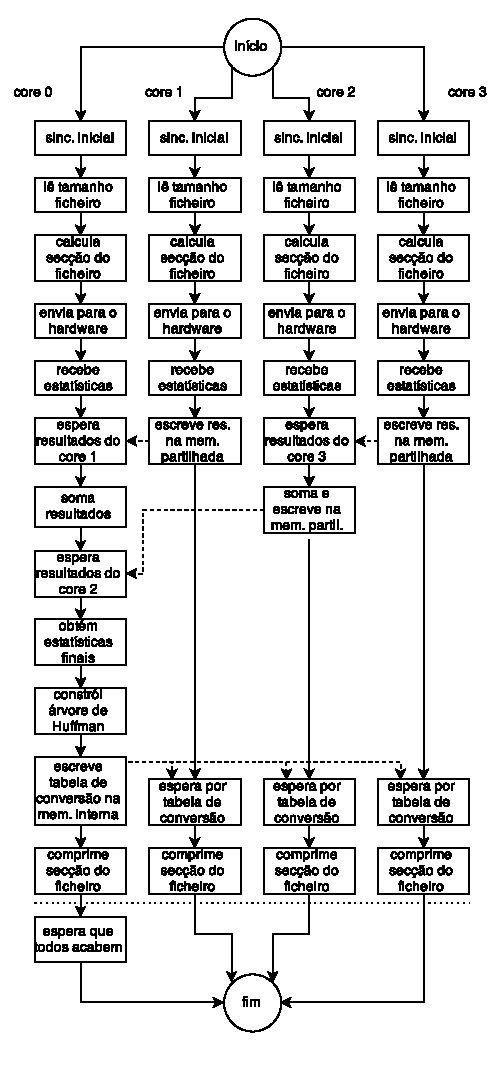
\includegraphics[height=0.95\textheight]{img/flowchart.pdf}
\caption{Fluxo de execução da aplicação}
\label{fig:software_flowchart}
\end{figure}